\documentclass{beamer}
\usetheme[hideothersubsections]{AUTheme}
\usefonttheme[]{serif}
\usepackage{pgf,pgfpages,pgfplots,epic,eepic}
\usepackage{graphicx}
\usepackage{amsmath, latexsym, color, amssymb, here}
\usepackage{epsf, epsfig, pifont,tikz,subfigure}
\usepackage{graphics, calrsfs}
\usepackage{times}
\usepackage{fancybox,calc}
\usepackage{palatino,mathpazo}
%------------------------------------------------------------
\title{More PGFplots}
\author{Jennifer Wang}
\institute{Department of Electrical and Computer Engineerig\\
						Auburn University}
\date{\today}
\begin{document}
\maketitle
\setbeamertemplate{footline}[page number]
%----------------------------------------------------------frame1
\section{Introduction to 3D plots using PGFPLOTS}
\begin{frame}	
	\frametitle{Introduction to 3D plots using PGFPLOTS}
	Why using PGFPLOTS for 3D plots\\
	\begin{itemize}
	\item Consistent fonts
	\item Consistent styles
	\item High-quality outputs
	\end{itemize}
\end{frame}
%------------------------------------------------------------frame2
\section{Draw backs of using PGFPLOTS for three dimensional plots}
\begin{frame}
	\frametitle{Draw backs of using PGFPLOTS for three dimensional plots}
  \begin{itemize}
	\item PGFPLOTS' three dimensional routines are slow.
  \item The plot complexity of three dimensional plots is limited to relatively coarse resolutions.
  \item PGFPLOTS supports z buffering techniques up to a certain extend.
  \end{itemize}
\end{frame}
%--------------------------------------------------------------frame3
\section{addplot3[options]{input data};}
\begin{frame}
	\frametitle{\color{blue}addplot3 \color{black}[options]\{input data\};}
	The \color{blue}{addplot3} \color{black}command accepts the same input methods as the \color{blue}{addplot} \color{black}variant, including coordinates, expression plotting, files and tables.
\end{frame}
%--------------------------------------------------------------frame4
\section{reading in a set of coordinates as input}
\begin{frame}[fragile]
   \frametitle{\color{blue}\textbackslash addplot3 coordinates \color{black} \{...\};}
   coordinates in form of matrix\\
   seperated by a line space\\
\begin{block}{Code}
\begin{verbatim}
\begin{tikzpicture}
		\begin{axis}
		\addplot[surf] coordinates{
(0,0,0) (1,0,0) (2,0,0) (3,0,0)

(0,1,0) (1,1,0.6) (2,1,0.7) (3,1,0.5)

(0,2,0) (1,2,0.7) (2,2,0.8) (3,2,0.5)
};	
		\end{axis}
		\end{tikzpicture}
\end{verbatim}
\end{block}
\end{frame}
%---------------------------------------------------------------frame5
\begin{frame}[fragile]
   \frametitle{\color{blue}\textbackslash addplot3 coordinates \color{black} \{...\};}
   coordinates in form of matrix\\
   seperated by \color{blue} \textbackslash par\\
\begin{block}{Code}
\begin{verbatim}
\begin{tikzpicture}
		\begin{axis}
		\addplot[surf] coordinates{
(0,0,0) (1,0,0) (2,0,0) (3,0,0)\par
(0,1,0) (1,1,0.6) (2,1,0.7) (3,1,0.5)\par
(0,2,0) (1,2,0.7) (2,2,0.8) (3,2,0.5)\par
};	
		\end{axis}
		\end{tikzpicture}
\end{verbatim}
\end{block}
\end{frame}   
%---------------------------------------------------------------frame6  
\begin{frame}[fragile]
   \frametitle{\color{blue}\textbackslash addplot3 coordinates \color{black} \{...\};}
   coordinates in form of matrix\\
   \color{blue} mesh \textbackslash rows \color{black}= \{interger\}\\
   \color{blue} mesh \textbackslash cols \color{black}= \{interger\}\\
\begin{block}{Code}
\begin{verbatim}
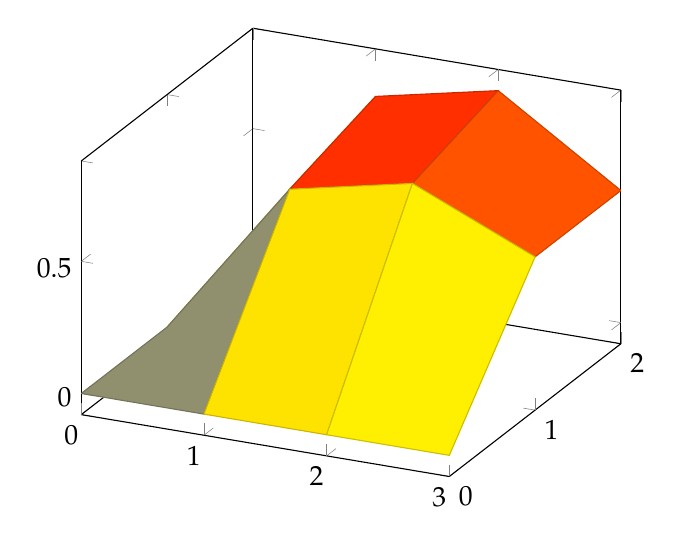
\begin{tikzpicture}
		\begin{axis}
		\addplot3[surf,mesh/rows=3] coordinates{
% this also yields a 3x4 matrix
(0,0,0) (1,0,0) (2,0,0) (3,0,0)
(0,1,0) (1,1,0.6) (2,1,0.7) (3,1,0.5)
(0,2,0) (1,2,0.7) (2,2,0.8) (3,2,0.5)
};
\end{axis}
\end{tikzpicture}
\end{verbatim}
\end{block}
\end{frame}   
%---------------------------------------------------------------frame7 
\begin{frame}[fragile]
   \frametitle{\color{blue}\textbackslash addplot3 coordinates \color{black} \{...\};}
\begin{block}{Plot}
\centering{
		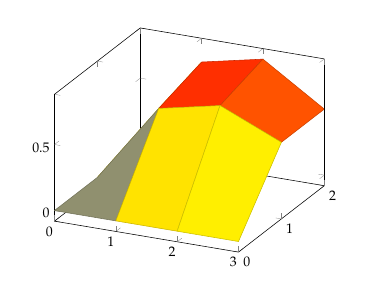
\begin{tikzpicture}[scale=0.5]
		\begin{axis}
		\addplot3[surf] coordinates{
(0,0,0) (1,0,0) (2,0,0) (3,0,0)

(0,1,0) (1,1,0.6) (2,1,0.7) (3,1,0.5)

(0,2,0) (1,2,0.7) (2,2,0.8) (3,2,0.5)
};
		\end{axis}
		\end{tikzpicture}
		}
\end{block}
\end{frame}
%---------------------------------------------------------------frame8 
\section{reading in a math expression as input}
\begin{frame}[fragile]
   \frametitle{\color{blue}\textbackslash addplot3 \color{black} \{math expression\};}
\begin{block}{Code}
\begin{verbatim}
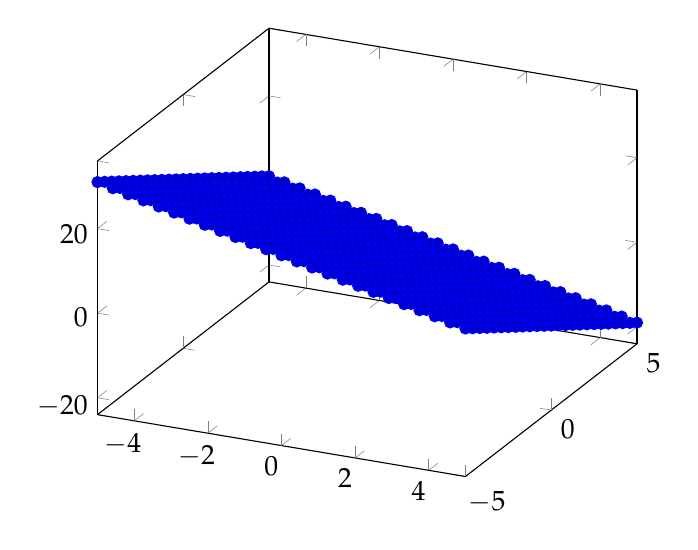
\begin{tikzpicture}
   \begin{axis}
    \addplot3{6-2*x-3*y}; 
   \end{axis}
\end{tikzpicture}
\end{verbatim}
\end{block}
\end{frame}
%---------------------------------------------------------------frame9
\begin{frame}[fragile]
\frametitle{\color{blue}\textbackslash addplot3 \color{black} \{math expression\};}
\begin{block}{Plot}
\centering{
		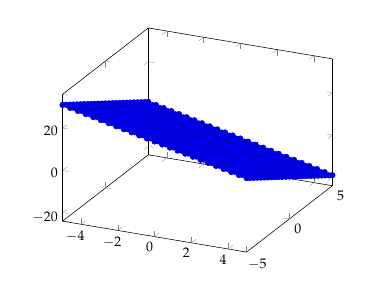
\begin{tikzpicture}[scale=0.5]
		\begin{axis}
		\addplot3{6-2*x-3*y}; 
		\end{axis}
		\end{tikzpicture}
		}
\end{block}
\end{frame}
%---------------------------------------------------------------frame10
\begin{frame}
   \frametitle{\color{blue}\textbackslash addplot3 \color{black} \{math expression\};}
controling plotting area:\\
\color{black} Interval[$x1$,$x2$]: \color{blue} domain\\
\color{black} Interval[$y1$,$y2$]: \color{blue} $y$ domain\\
\vspace{30pt}
\color{black} controling number of samples:\\ 
\color{black} Number of samples in $x$ direction: \color{blue} samples\\
\color{black} Number of samples in $y$ direction: \color{blue} samples $y$\\
\end{frame}
%---------------------------------------------------------------frame11
\begin{frame}[fragile]
   \frametitle{\color{blue}\textbackslash addplot3 \color{black} \{math expression\};}
\begin{block}{Code}
\begin{verbatim}
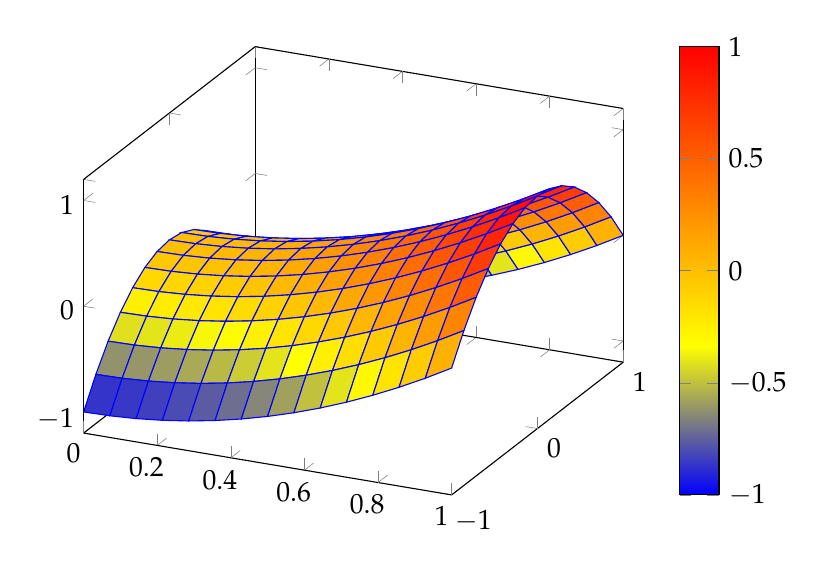
\begin{tikzpicture}
\begin{axis}[colorbar]
\addplot3
[surf,faceted color=blue,
 samples=15,
 domain=0:1,y domain=-1:1]
{x^2 - y^2};
\end{axis}
\end{tikzpicture}
\end{verbatim}
\end{block}
\end{frame}
%---------------------------------------------------------------frame12
\begin{frame}[fragile]
\frametitle{\color{blue}\textbackslash addplot3 \color{black} \{math expression\};}
\begin{block}{Plot}
\centering{
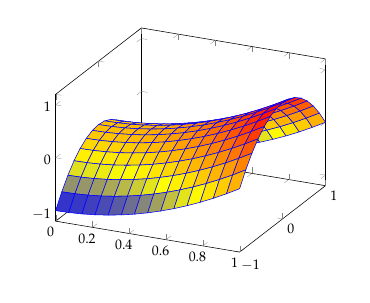
\begin{tikzpicture}[scale=0.5]
\begin{axis}
\addplot3
[surf,faceted color=blue, samples=15, domain=0:1,y domain=-1:1]
{x^2 - y^2};
\end{axis}
\end{tikzpicture}
}
\end{block}
\end{frame}
%---------------------------------------------------------------frame13
\section{reading in a file as input}
\begin{frame}[fragile]
\frametitle{\color{blue}\textbackslash addplot file \color{black} \{file name\};}
\begin{itemize}
\item generating file by notepad
\item saving as .dat file
\item needing to have at least 2 columns for 2D and 3 columns for 3D
\item lines starting with \% and \# are ignored
\end{itemize}
\end{frame}
%---------------------------------------------------------------frame14
\begin{frame}[fragile]
\frametitle{\color{blue}\textbackslash addplot file \color{black} \{file name\};}
\begin{block}{Code}
\begin{verbatim}
\begin{axis}
\addplot file {plotdata.dat};
\end{axis}
\end{tikzpicture}
\end{verbatim}
\end{block}
\begin{block}{plotdata.dat}
\begin{verbatim}
0 1
1 2
2 3
3 4
4 5
6 7
\end{verbatim}
\end{block}
\end{frame}
%---------------------------------------------------------------frame15
\begin{frame}[fragile]
\frametitle{\color{blue}\textbackslash addplot file \color{black} \{file name\};}
\begin{block}{Plot}
\centering{
\begin{tikzpicture}[scale=0.5]
\begin{axis}
\addplot file {plotdata.dat};
\end{axis}
\end{tikzpicture}
}
\end{block}
\end{frame}
%---------------------------------------------------------------frame16
\section{reading in a table as input}
\begin{frame}[fragile]
\frametitle{\color{blue}\textbackslash addplot table \color{black} [column selection] \{file\};}
\begin{itemize}
\item \color{blue} plot table \color{black} similar to \color{blue} plot file \color{black} .
\item generating file by notepad
\item saving as .dat file
\item multiple columns
\item plotting certain columns
\end{itemize}
\end{frame}
%---------------------------------------------------------------frame17
\begin{frame}[fragile]
\frametitle{\color{blue}\textbackslash addplot table \color{black} [column selection] \{file\};}
\begin{block}{Code}
\begin{verbatim}
\begin{axis}
\addplot table[x=a,y=c] {plottable.dat};
\end{axis}
\end{tikzpicture}
\end{verbatim}
\end{block}
\begin{block}{plottable.dat}
\begin{verbatim}
a b c
0 1 2
2 3 4
4 5 6
6 7 8
8 9 10
\end{verbatim}
\end{block}
\end{frame}
%---------------------------------------------------------------frame18
\begin{frame}[fragile]
\frametitle{\color{blue}\textbackslash addplot table \color{black} [column selection] \{file\};}
\begin{block}{Plot}
\centering{
\begin{tikzpicture}[scale=0.5]
\begin{axis}
\addplot table[x=a,y=c] {plottable.dat};
\end{axis}
\end{tikzpicture}
}
\end{block}
\end{frame}
%---------------------------------------------------------------frame19
\section{line plots as output}
\begin{frame}[fragile]
\frametitle{line plots for coordinates input}
generated if input source has no matrix structure\\
\vspace{30pt}
\small{
\begin{block}{Code}
\begin{verbatim}
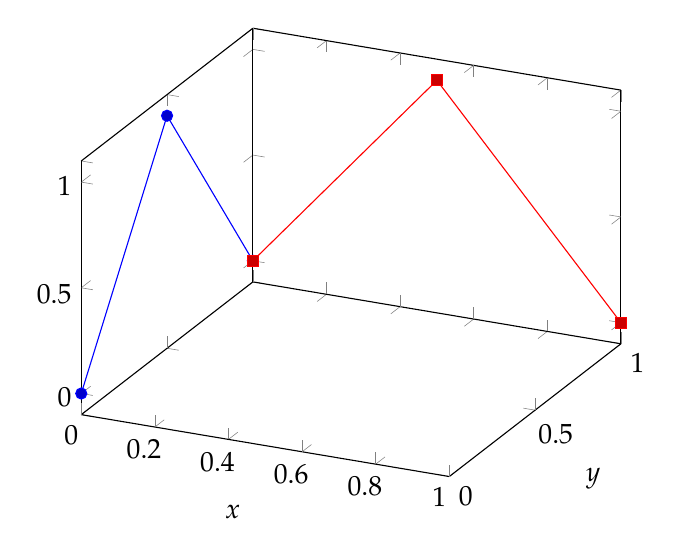
\begin{tikzpicture}
\begin{axis}[xlabel=$x$,ylabel=$y$]
\addplot3 coordinates{(0,0,0)(0,0.5,1)(0,1,0)};
\addplot3 coordinates{(0,1,0)(0.5,1,1)(1,1,0)};
\end{axis}
\end{tikzpicture}
\end{verbatim}
\end{block}}
\end{frame}
%---------------------------------------------------------------frame20
\begin{frame}[fragile]
\frametitle{line plots:generated if input source has no matrix structure}
\begin{block}{Plot}
\centering{
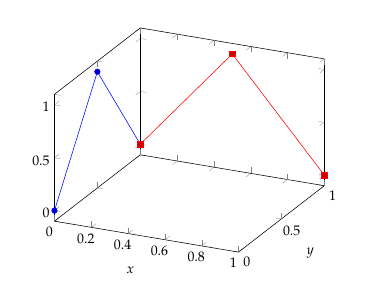
\begin{tikzpicture}[scale=0.5]
\begin{axis}[xlabel=$x$,ylabel=$y$]
\addplot3 coordinates{(0,0,0)(0,0.5,1)(0,1,0)};
\addplot3 coordinates{(0,1,0)(0.5,1,1)(1,1,0)};
\end{axis}
\end{tikzpicture}
}
\end{block}
\end{frame}
%---------------------------------------------------------------frame21
\begin{frame}[fragile]
\frametitle{line plots for expression input}
set \color{blue} samples y=0 \color{black} to disable the generation of a mesh\\
\vspace{30pt}
\small{
\begin{block}{Code}
\begin{verbatim}
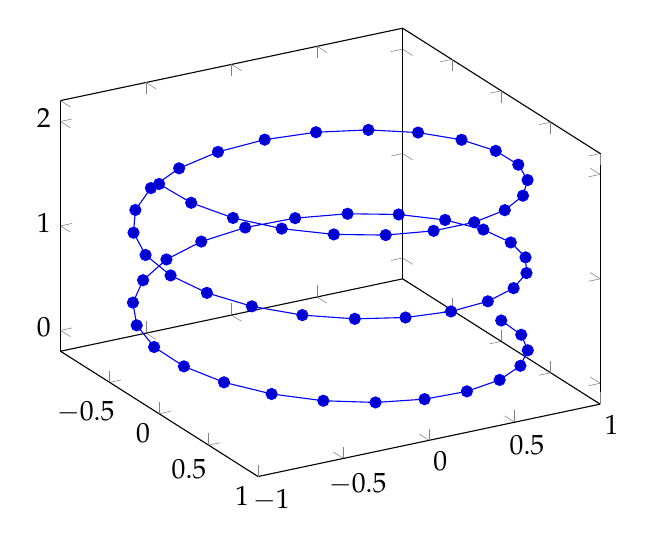
\begin{tikzpicture}
\begin{axis}[view={60}{30}]
\addplot3+[domain=0:5*pi,samples=60,samples y=0]
({sin(deg(x))},
{cos(deg(x))},
{2*x/(5*pi)});
\end{axis}
\end{tikzpicture}
\end{verbatim}
\end{block}}
\end{frame}
%---------------------------------------------------------------frame22
\begin{frame}[fragile]
\frametitle{line plots for expression input}
\begin{block}{Plot}
\centering{
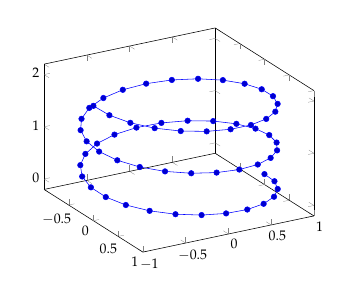
\begin{tikzpicture}[scale=0.5]
\begin{axis}[view={60}{30}]
\addplot3+[domain=0:5*pi,samples=60, samples y=0]
({sin(deg(x))},
{cos(deg(x))},
{2*x/(5*pi)});
\end{axis}
\end{tikzpicture}
}
\end{block}
\end{frame}
%---------------------------------------------------------------frame23
\begin{frame}[fragile]
\color{blue} addplot \color{black} + [options] does the same as \color{blue} addplot \color{black} [options]; except that [options] are appended to the arguments which would have been taken for \color{blue} addplot \color{black} (the element of the default list).
\end{frame}
%---------------------------------------------------------------frame24
\section{mesh plots as output}
\begin{frame}
\frametitle{How does mesh plot work}
\begin{itemize}
\item A mesh plot uses different color for each mesh segment. Each mesh segment gets the same color. 
\item The colour is determined using a color coordinate. In the initial configuration, the color coordinate is the z axis.
\item This color coordinate is mapped linearly into the current color map to determine the color for each mesh segment.
\item This works the same for surface plots and scatter plots.
\end{itemize}
\end{frame}
%---------------------------------------------------------------frame25
\begin{frame}[fragile]
\frametitle{\color{blue} addplot3[mesh]}
\begin{block}{Code}
\begin{verbatim}
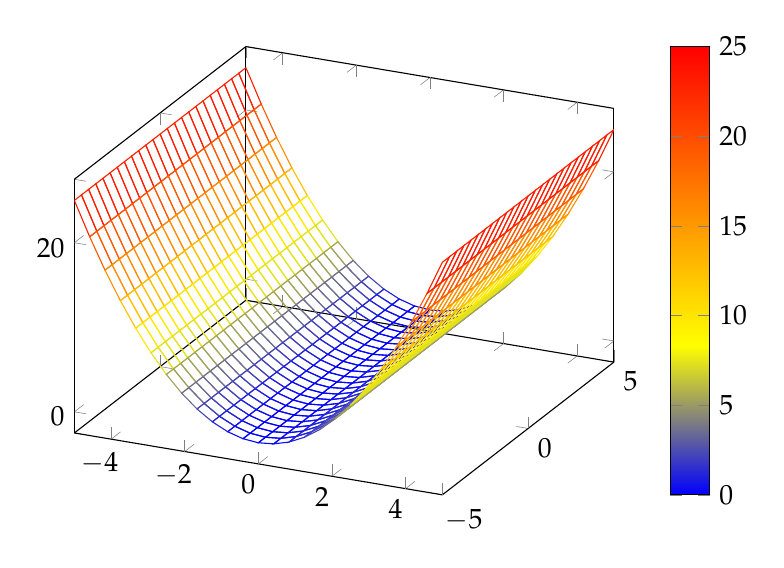
\begin{tikzpicture}
\begin{axis}[colorbar]
\addplot3[mesh] {x^2};
\end{axis}
\end{tikzpicture}
\end{verbatim}
\end{block}
\end{frame}
%---------------------------------------------------------------frame26
\begin{frame}[fragile]
\frametitle{\color{blue} addplot3[mesh]}
\begin{block}{Plot}
\centering{
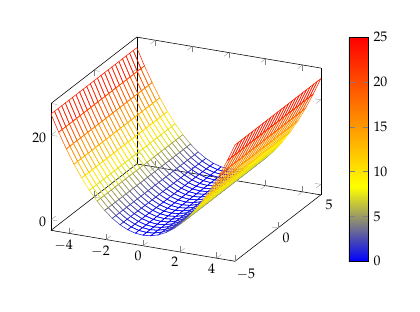
\begin{tikzpicture}[scale=0.5]
\begin{axis}[colorbar]
\addplot3[mesh] {x^2};
\end{axis}
\end{tikzpicture}
}
\end{block}
\end{frame}
%---------------------------------------------------------------frame27
\begin{frame}[fragile]
\frametitle{\color{blue} addplot3[mesh]}
A mesh plot can be combined with markers or with the scatter key to draw markers in different colors.
\vspace{20pt}
\begin{block}{Code}
\begin{verbatim}
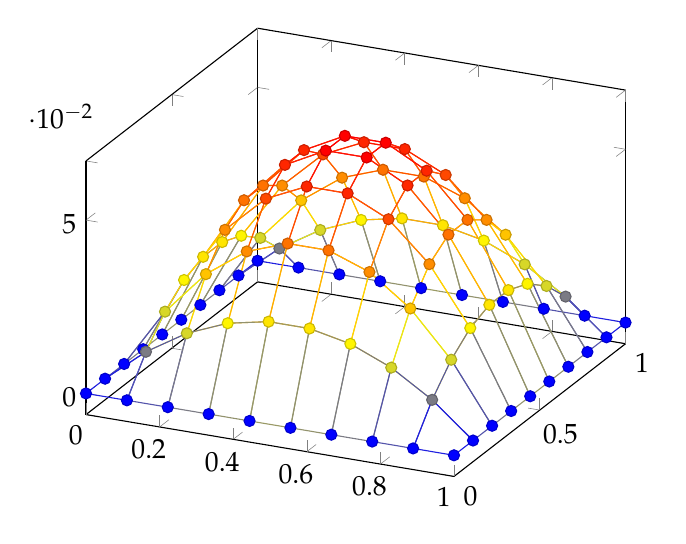
\begin{tikzpicture}
\begin{axis}
\addplot3+[mesh,scatter,
           samples=10,domain=0:1]
{x*(1-x)*y*(1-y)};
\end{axis}
\end{tikzpicture}
\end{verbatim}
\end{block}
\end{frame}
%---------------------------------------------------------------frame28
\begin{frame}[fragile]
\frametitle{\color{blue} addplot3[mesh]}
\begin{block}{Plot}
\centering{
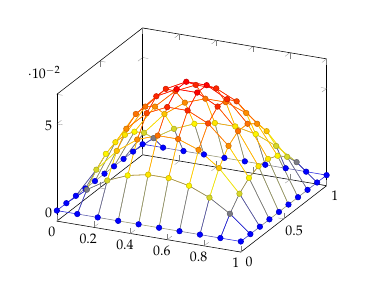
\begin{tikzpicture}[scale=0.5]
\begin{axis}
\addplot3+[mesh,scatter,samples=10,domain=0:1]
{x*(1-x)*y*(1-y)};
\end{axis}
\end{tikzpicture}
}
\end{block}
\end{frame}
%---------------------------------------------------------------frame29
\section{surface plots as output}
\begin{frame}[fragile]
\frametitle{\color{blue} addplot3[surf]}
\begin{block}{Code}
\begin{verbatim}
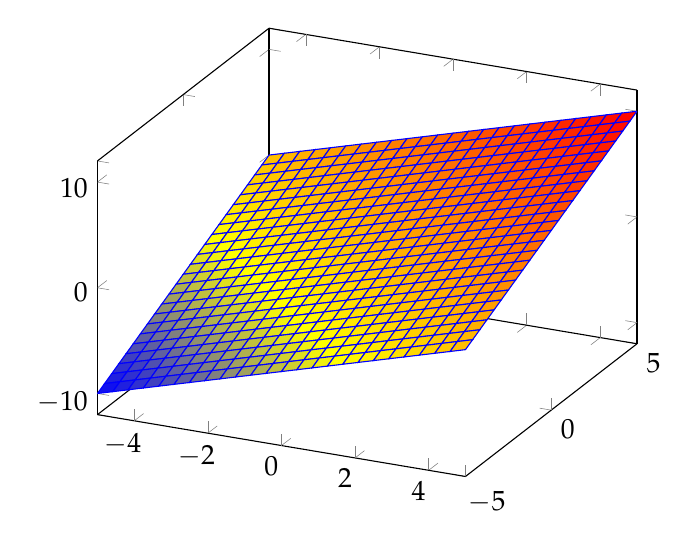
\begin{tikzpicture}
\begin{axis}
\addplot3[surf,faceted color=blue] {x+y};
\end{axis}
\end{tikzpicture}
\end{verbatim}
\end{block}
\end{frame}
%---------------------------------------------------------------frame30
\begin{frame}[fragile]
\frametitle{\color{blue} addplot3[surf]}
\begin{block}{Plot}
\centering{
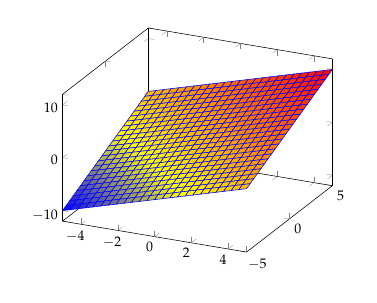
\begin{tikzpicture}[scale=0.5]
\begin{axis}
\addplot3[surf,faceted color=blue] {x+y};
\end{axis}
\end{tikzpicture}
}
\end{block}
\end{frame}
%---------------------------------------------------------------frame31
\section{z buffer}
\begin{frame}[fragile]
\frametitle{How does z buffer work}
\begin{itemize}
\item A z buffer determines which parts of an image should be drawn in front of other parts.
\item The z buffering algorithms of pgfplots apply only to a single \color{blue}addplot \color{black}command. Different \color{blue} addplot \color{black} commands will be drawn on top of each other, in the order of appearance.
\item The choice \color{blue} default \color{black} checks if we are currently working with a mesh or surface plot and uses \color{blue} auto \color{black} in this case. If not, it sets \color{blue} z buffer=none \color{black}.
\item The choice \color{blue} none \color{black} disables z buffering. This is also the case for two dimensional axes which don't need z buffering.
\end{itemize}
\end{frame}
%---------------------------------------------------------------frame32
\section{Markers}
\begin{frame}[fragile]
\frametitle{Different styles of markers}
\begin{figure}
\centering
\includegraphics[width=0.8\textwidth]{fig1.jpg}
\end{figure}
\end{frame}
%---------------------------------------------------------------frame33
\begin{frame}[fragile]
\frametitle{More styles of markers}
\begin{figure}
\centering
\includegraphics[width=0.8\textwidth]{fig2.jpg}
\end{figure}
\end{frame}
%---------------------------------------------------------------frame34
\begin{frame}[fragile]
\frametitle{An example of using different marks}
\begin{block}{Code}
\begin{verbatim}
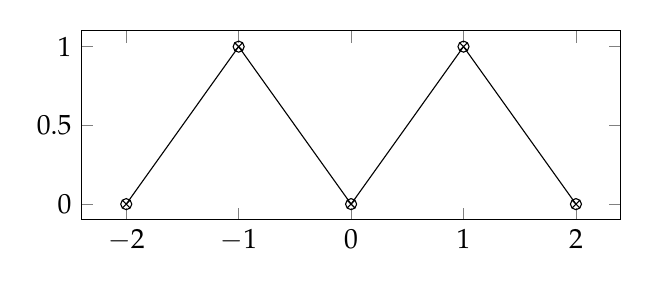
\begin{tikzpicture}
\begin{axis}[y=2cm]
\addplot [mark=otimes] coordinates
{(-2,0) (-1,1) (0,0) (1,1) (2,0)};
\end{axis}
\end{tikzpicture}
\tikzset{every mark/.append style={scale=2,
mark=otimes}}
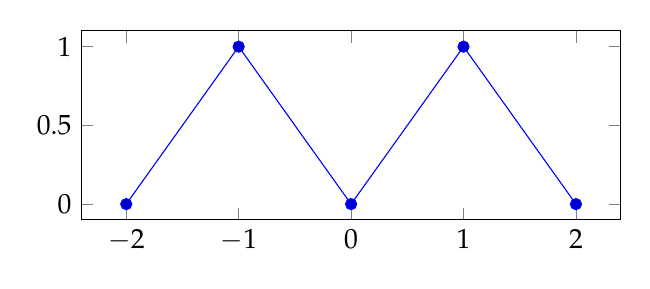
\begin{tikzpicture}
\begin{axis}[y=2cm,mark=otimes]
\addplot coordinates
{(-2,0) (-1,1) (0,0) (1,1) (2,0)};
\end{axis}
\end{tikzpicture}
\end{verbatim}
\end{block}
\end{frame}
%---------------------------------------------------------------frame35
\begin{frame}[fragile]
\frametitle{An example of using different marks}
\begin{block}{Plot}
\centering{
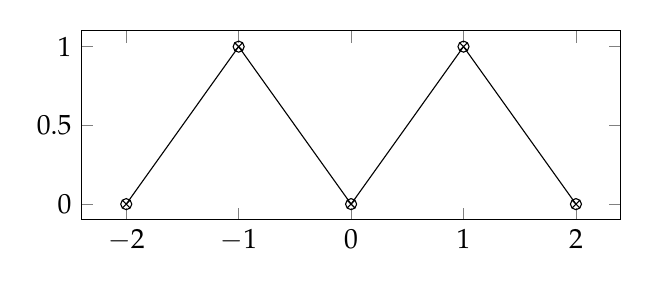
\begin{tikzpicture}
\begin{axis}[y=2cm]
\addplot [mark=otimes] coordinates
{(-2,0) (-1,1) (0,0) (1,1) (2,0)};
\end{axis}
\end{tikzpicture}
\tikzset{every mark/.append style={scale=2,mark=otimes}}
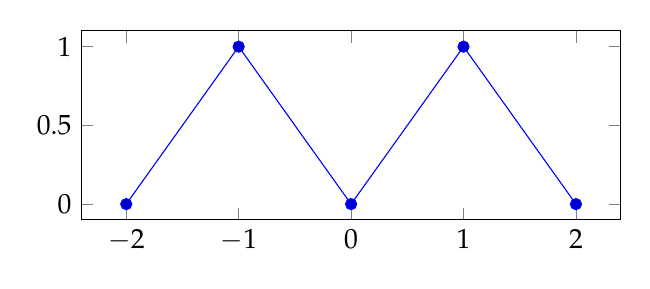
\begin{tikzpicture}
\begin{axis}[y=2cm]
\addplot coordinates
{(-2,0) (-1,1) (0,0) (1,1) (2,0)};
\end{axis}
\end{tikzpicture}
}
\end{block}
\end{frame}
%---------------------------------------------------------------frame36
\section{Line styles}
\begin{frame}[fragile]
\frametitle{Different styles of lines}
\begin{figure}
\centering
\includegraphics[width=0.8\textwidth]{fig3.jpg}
\end{figure}
\end{frame}
%---------------------------------------------------------------frame37
\begin{frame}[fragile]
\frametitle{An example of using different line styles}
\begin{block}{Code}
\begin{verbatim}
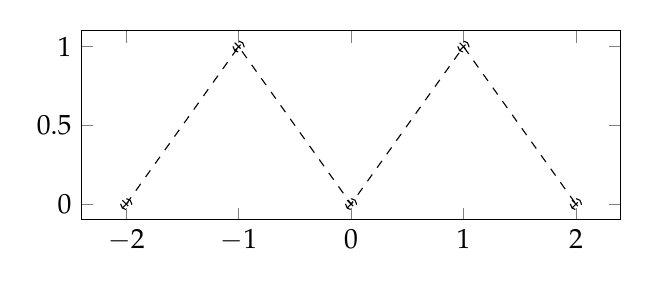
\begin{tikzpicture}
\begin{axis}[y=2cm]
\addplot[mark=otimes,dashed] coordinates
{(-2,0) (-1,1) (0,0) (1,1) (2,0)};
\end{axis}
\end{tikzpicture}
\end{verbatim}
\end{block}
\end{frame}
%---------------------------------------------------------------frame38
\begin{frame}[fragile]
\frametitle{An example of using different line styles}
\begin{block}{Plot}
\centering{
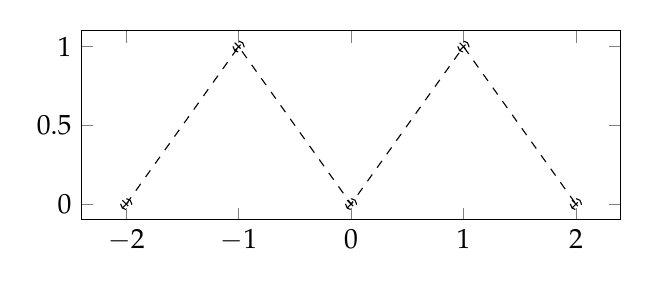
\begin{tikzpicture}
\begin{axis}[y=2cm]
\addplot[mark=otimes,dashed] coordinates
{(-2,0) (-1,1) (0,0) (1,1) (2,0)};
\end{axis}
\end{tikzpicture}
}
\end{block}
\end{frame}
%---------------------------------------------------------------frame39
\begin{frame}[fragile]
\frametitle{Line width}
\begin{itemize}
\item thin
\item ultra thin
\item very thin
\item semithick
\item thick
\item very thick
\item ultra thick
\end{itemize}
\end{frame}
%---------------------------------------------------------------frame40
\section{Font size}
\begin{frame}[fragile]
\frametitle{Font size}
\begin{itemize}
\item Sets the font which is to be used for text in nodes (like tick labels, legends or descriptions).
\item A font can be any \LaTeX\ argument like \color{blue} footnotesize \color{black} or \color{blue} small \textbackslash bfseries.
\end{itemize}
\end{frame}
%---------------------------------------------------------------frame41
\section{Colors}
\begin{frame}[fragile]
\frametitle{Colors}
\begin{itemize}
\item The package xcolor defines a set of predefined colors, namely red, green, blue, cyan,magenta, yellow, black, gray, white, darkgray, lightgray, brown, lime,olive, orange, pink, purple, teal, violet.
\item Besides predefined colors, it is possible to mix two (or more) colors. For example, red!30!white contains 30\% of red and 70\% of white. Consequently, one can build red!70!white to get 70\% red and 30\% white or red!10!white for 10\% red and 90\% white.
\item A different type of color mixing is supported, which allows to take 100\% of each component. For example, rgb,2:red,1;green,1 will add 1/2 part red and 1/2 part green.
\end{itemize}
\end{frame}
%---------------------------------------------------------------frame42
\section{Color Maps}
\begin{frame}[fragile]
\frametitle{Color Maps}
\begin{itemize}
\item By using commands\\
\color{blue} colormap name \color{black} = \{color map name\} or \color{blue} colormap \textbackslash \color{black} a kind of colormap, it changes the current color map to the already defined map named.
\item The predefined color map is hot.
\end{itemize}
\end{frame}
%---------------------------------------------------------------frame43
\begin{frame}[fragile]
\frametitle{Different color maps}
\begin{itemize}
\item hot
\begin{figure}
\centering
\includegraphics[width=0.8\textwidth]{fig4.jpg}
\end{figure}
\item bluered
\item cool
\item greenyellow
\item redyellow
\item violet
\item blackwhite
\end{itemize}
\end{frame}
%---------------------------------------------------------------frame44
\section{Axis background}
\begin{frame}[fragile]
\frametitle{An example of using a different axis background}
\begin{block}{Code}
\begin{verbatim}
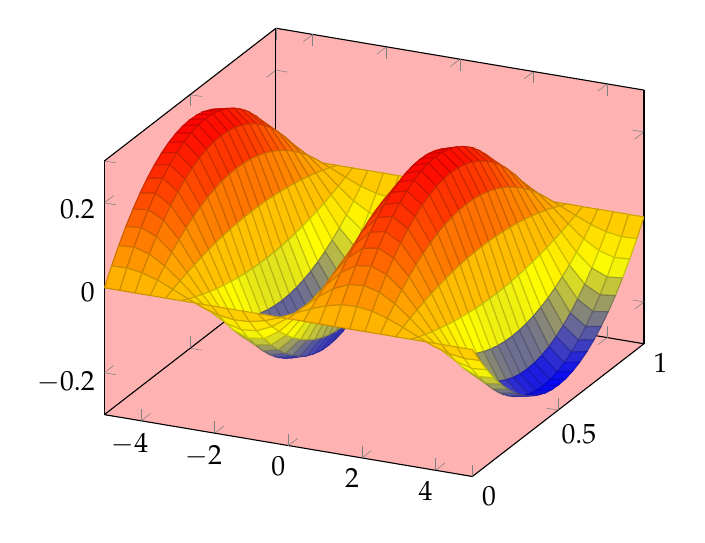
\begin{tikzpicture}
\begin{axis}[
axis background/.style={fill=red!30!white}]
\addplot3[surf,y domain=0:1]
{sin(deg(x)) * y*(1-y)};
\end{axis}
\end{tikzpicture}
\end{verbatim}
\end{block}
\end{frame}
%---------------------------------------------------------------frame45
\section{Axis configuration}
\begin{frame}[fragile]
\frametitle{An example of using a different axis background}
\begin{block}{Plot}
\centering{
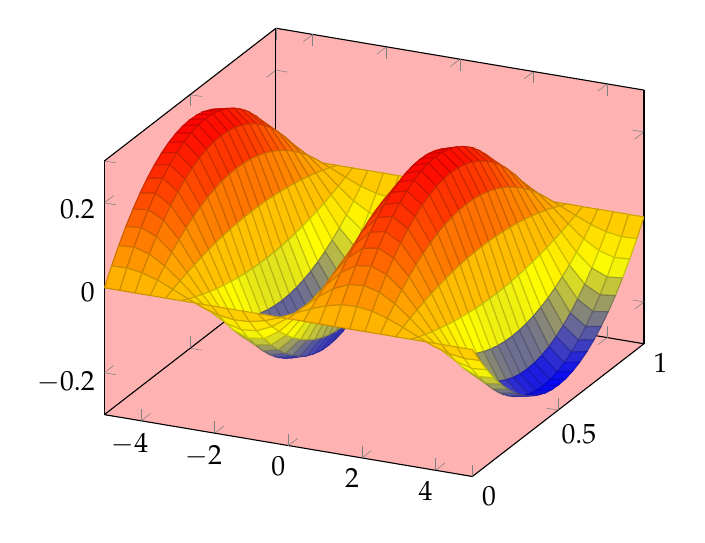
\begin{tikzpicture}
\begin{axis}[
axis background/.style={fill=red!30!white}]
\addplot3[surf,y domain=0:1]
{sin(deg(x)) * y*(1-y)};
\end{axis}
\end{tikzpicture}
}
\end{block}
\end{frame}
%---------------------------------------------------------------frame46
\section{Scaling options}
\begin{frame}[fragile]
\frametitle{width=\{ \}}
Sets the width of the final picture to \{ \}. If no height is specified, scaling will respect aspect ratios.
\begin{block}{Code}
\begin{verbatim}
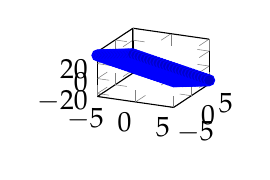
\begin{tikzpicture}
\begin{axis}[width=3cm]
\addplot3{6-2*x-3*y};
\end{axis}
\end{tikzpicture}
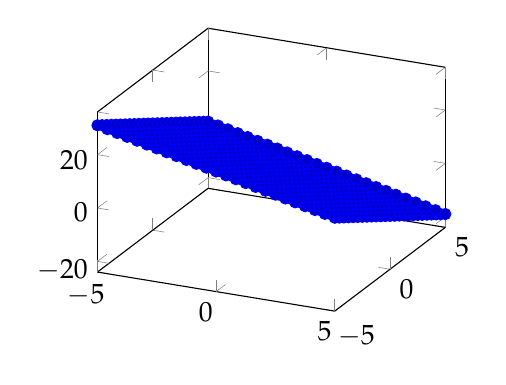
\begin{tikzpicture}
\begin{axis}[width=6cm]
\addplot3{6-2*x-3*y};
\end{axis}
\end{tikzpicture}
\end{verbatim}
\end{block}
\end{frame}
%---------------------------------------------------------------frame47
\begin{frame}[fragile]
\frametitle{width=\{ \}}
\begin{block}{Plot}
\centering{
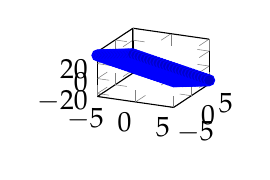
\begin{tikzpicture}
\begin{axis}[width=3cm]
\addplot3{6-2*x-3*y};
\end{axis}
\end{tikzpicture}
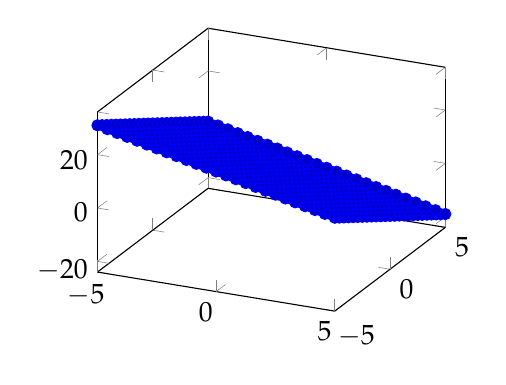
\begin{tikzpicture}
\begin{axis}[width=6cm]
\addplot3{6-2*x-3*y};
\end{axis}
\end{tikzpicture}
}
\end{block}
\end{frame}
%---------------------------------------------------------------frame48
\begin{frame}[fragile]
\frametitle{scale=\{number\}}
\color{blue} width=\{ \} \color{black} only affects the width of one unit in x-direction or the height for one unit in y-direction. Axis labels and tick labels won't be resized.\\
We can use the \color{blue} scale=\{\color{black}number\color{blue}\} \color{black} option to scale the complete picture.
\small{
\begin{block}{Code}
\begin{verbatim}
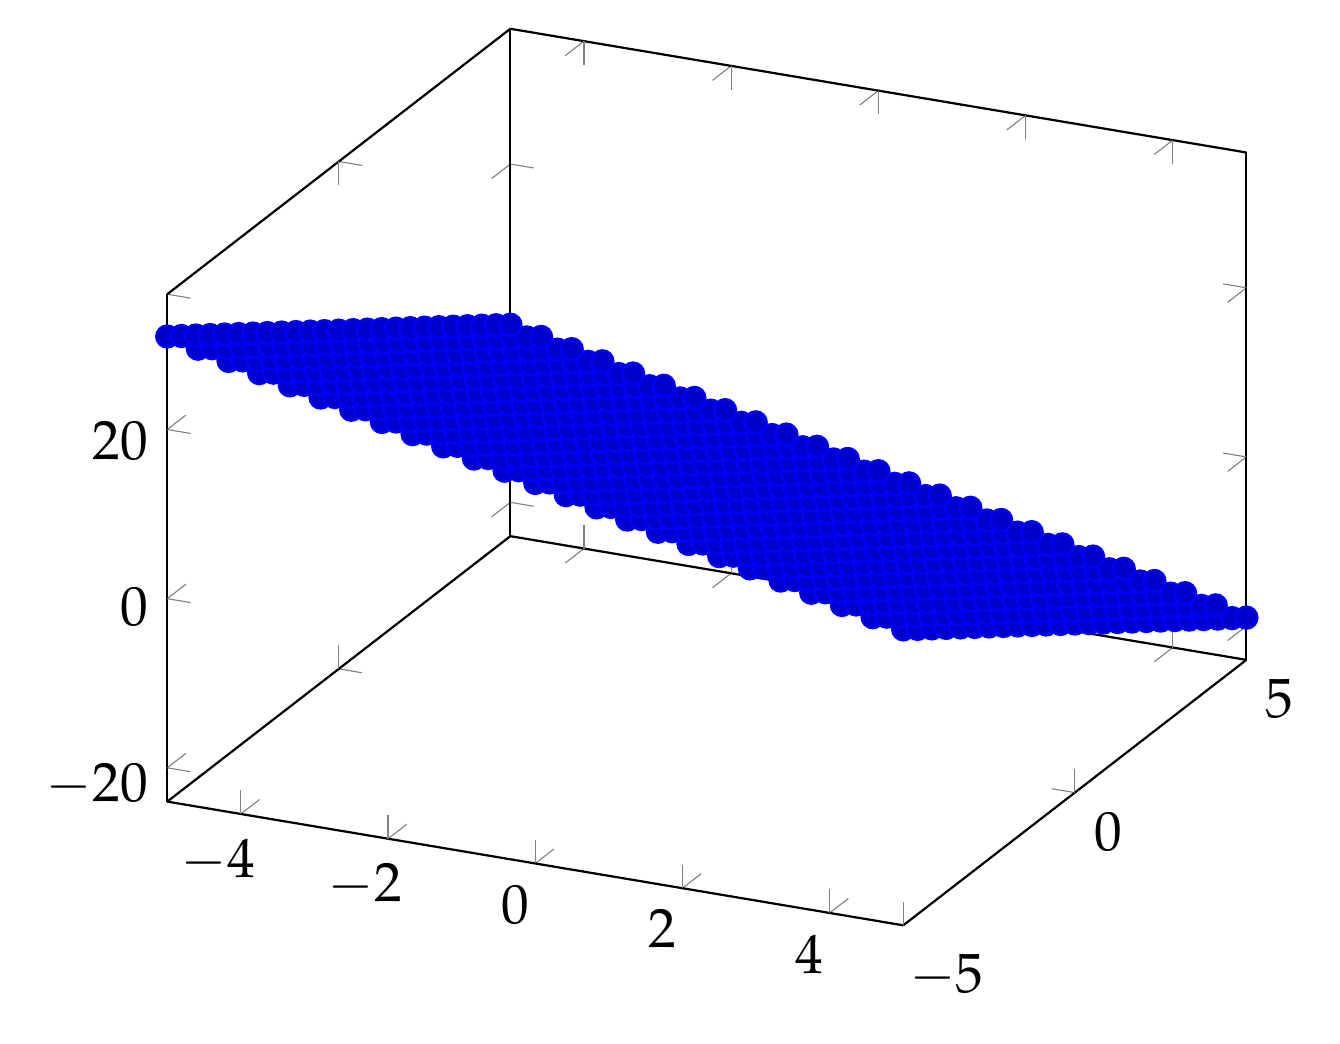
\begin{tikzpicture}[scale=2]
\begin{axis}
\addplot3{6-2*x-3*y};
\end{axis}
\end{tikzpicture}
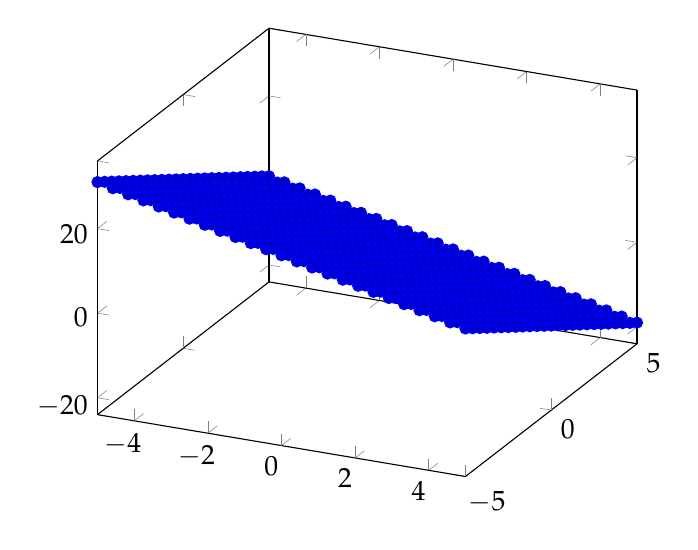
\begin{tikzpicture}
\begin{axis}
\addplot3{6-2*x-3*y};
\end{axis}
\end{tikzpicture}
\end{verbatim}
\end{block}}
\end{frame}
%---------------------------------------------------------------frame49
\begin{frame}[fragile]
\frametitle{scale=\{number\}}
\begin{block}{Plot scale=2}
\centering{
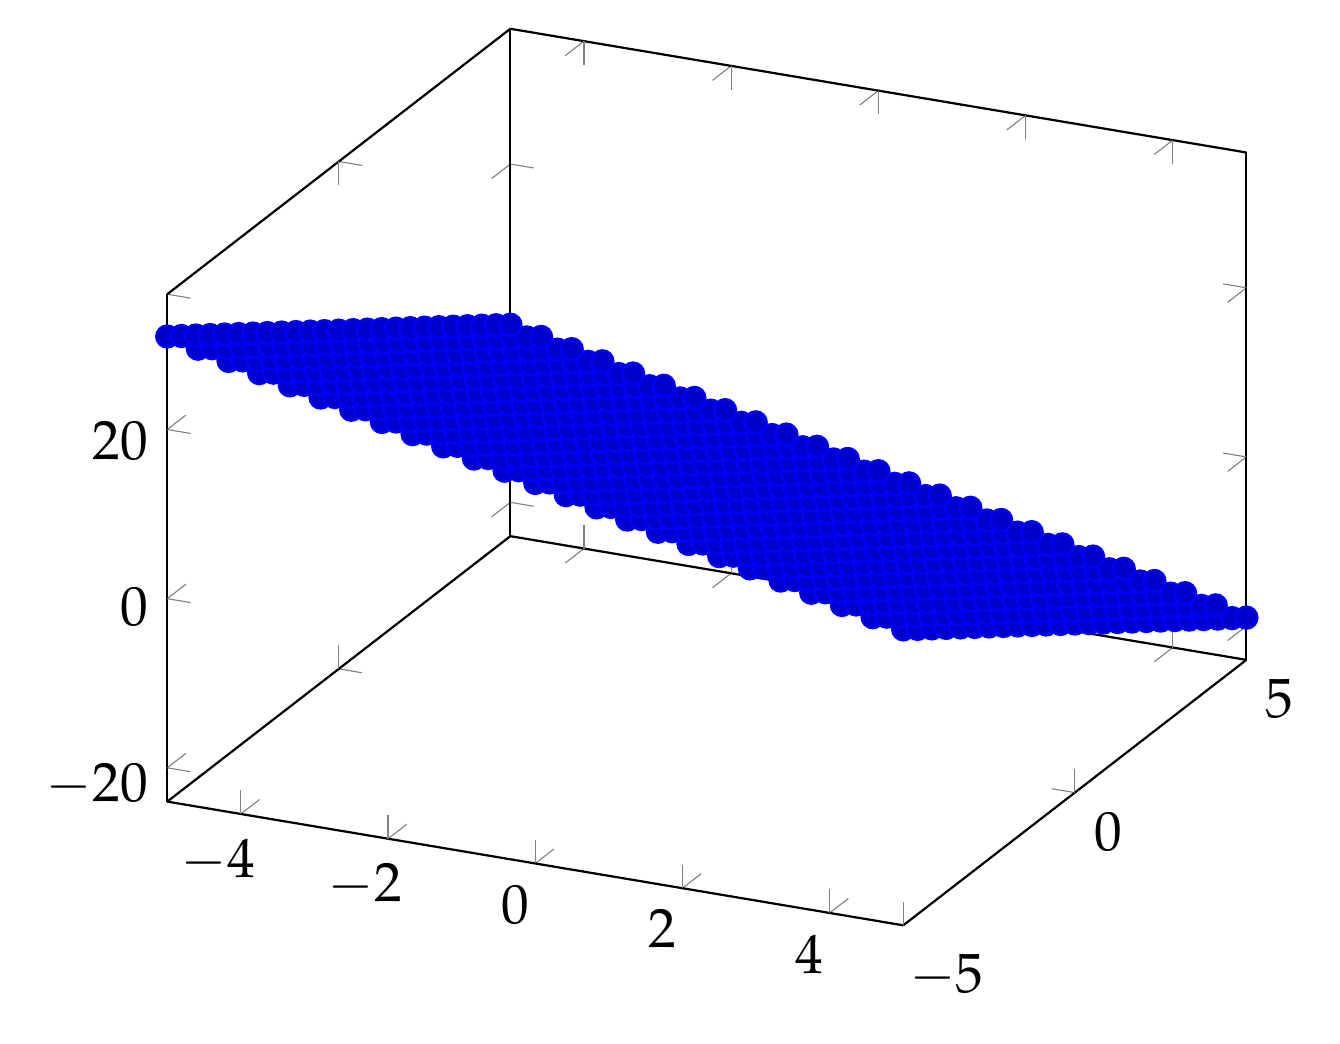
\begin{tikzpicture}[scale=2]
\begin{axis}
\addplot3{6-2*x-3*y};
\end{axis}
\end{tikzpicture}}
\end{block}
\end{frame}
%---------------------------------------------------------------frame50
\begin{frame}[fragile]
\frametitle{scale=\{number\}}
\begin{block}{Plot no scaling}
\centering{
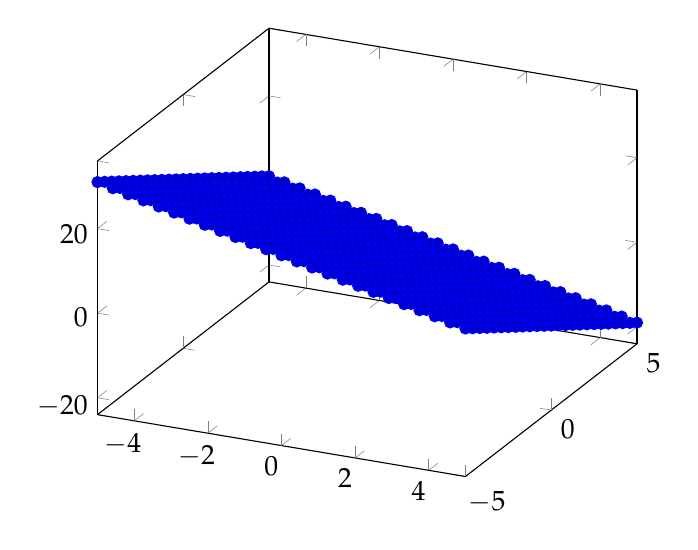
\begin{tikzpicture}
\begin{axis}
\addplot3{6-2*x-3*y};
\end{axis}
\end{tikzpicture}}
\end{block}
\end{frame}
%---------------------------------------------------------------frame51
\section{3D view configuration}
\begin{frame}[fragile]
\frametitle{3D view configuration}
\begin{itemize}
\item use command \color{blue} view \color{black} = \{ azimuth \} \{ elevation \}.
\item The azimuth (first argument) is the horizontal angle which is rotated around the $z$ axis.
\item The elevation (second argument) is the vertical rotation around the (rotated) $x$ axis.
\item Default value is \{25\}\{30\}.
\end{itemize}
\end{frame}
%---------------------------------------------------------------frame52
\begin{frame}[fragile]
\frametitle{\color{blue} view \color{black} = \{ azimuth \} \{ elevation \}}
\begin{block}{Code}
\begin{verbatim}
\begin{tikzpicture}
\begin{axis}[view={0}{0},
xlabel=$x$,
zlabel=$z$,
title=View along the positive $y$ axis]
\addplot3[surf] {x};
\end{axis}
\end{tikzpicture}
\end{verbatim}
\end{block}
\end{frame}
%---------------------------------------------------------------frame53
\begin{frame}[fragile]
\frametitle{\color{blue} view \color{black} = \{ azimuth \} \{ elevation \}}
\begin{block}{Plot}
\centering{
\begin{tikzpicture}
\begin{axis}[view={0}{0},
xlabel=$x$,
zlabel=$z$,
title=View along the positive $y$ axis]
\addplot3[surf] {x};
\end{axis}
\end{tikzpicture}}
\end{block}
\end{frame}
%---------------------------------------------------------------frame54
\begin{frame}[fragile]
\frametitle{\color{blue} view \color{black} = \{ azimuth \} \{ elevation \}}
\begin{block}{Code}
\begin{verbatim}
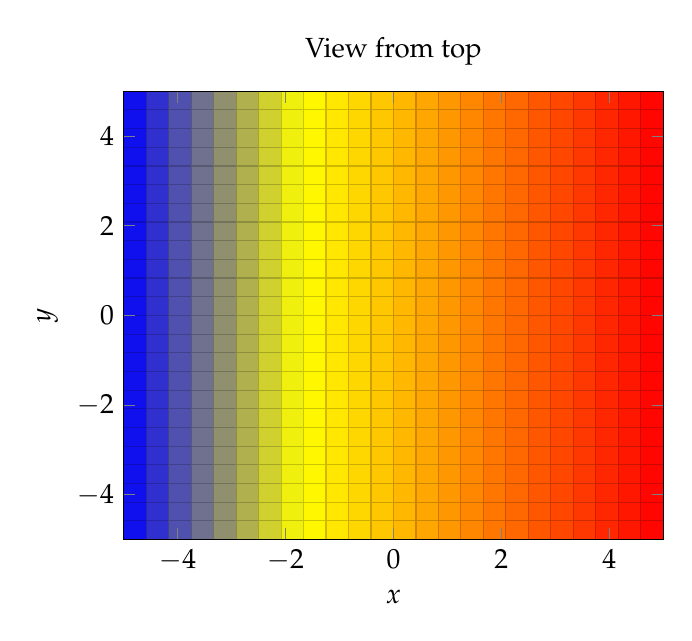
\begin{tikzpicture}
\begin{axis}[view={0}{90},
xlabel=$x$,
ylabel=$y$,
title=View from top]
\addplot3[surf] {x};
\end{axis}
\end{tikzpicture}
\end{verbatim}
\end{block}
\end{frame}
%---------------------------------------------------------------frame55
\begin{frame}[fragile]
\frametitle{\color{blue} view \color{black} = \{ azimuth \} \{ elevation \}}
\begin{block}{Plot}
\centering{
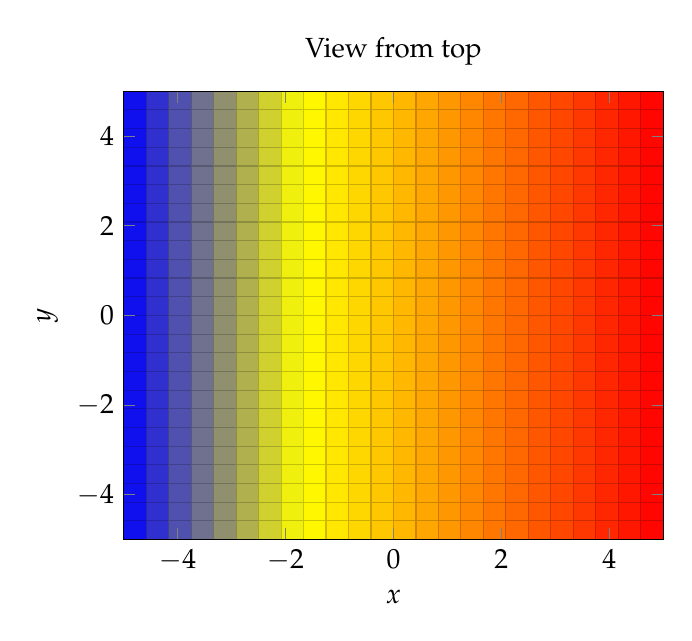
\begin{tikzpicture}
\begin{axis}[view={0}{90},
xlabel=$x$,
ylabel=$y$,
title=View from top]
\addplot3[surf] {x};
\end{axis}
\end{tikzpicture}}
\end{block}
\end{frame}
%---------------------------------------------------------------frame56
\begin{frame}[fragile]
\frametitle{\color{blue} view \color{black} = \{ azimuth \} \{ elevation \}}
\begin{block}{Code}
\begin{verbatim}
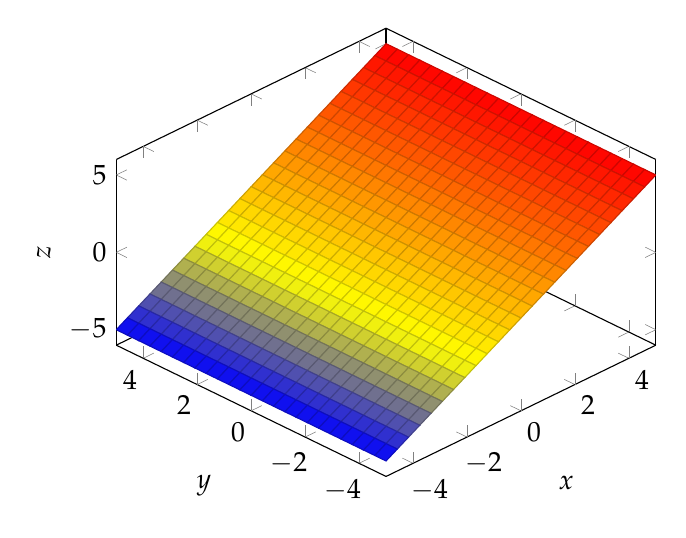
\begin{tikzpicture}
\begin{axis}[view={-45}{45},
xlabel=$x$,ylabel=$y$,zlabel=$z$]
\addplot3[surf] {x};
\end{axis}
\end{tikzpicture}
\end{verbatim}
\end{block}
\end{frame}
%---------------------------------------------------------------frame57
\begin{frame}[fragile]
\frametitle{\color{blue} view \color{black} = \{ azimuth \} \{ elevation \}}
\begin{block}{Plot}
\centering{
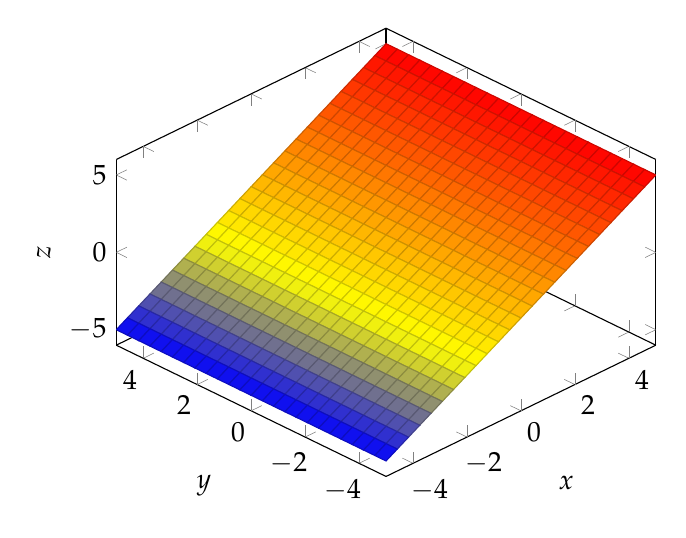
\begin{tikzpicture}
\begin{axis}[view={-45}{45},
xlabel=$x$,ylabel=$y$,zlabel=$z$]
\addplot3[surf] {x};
\end{axis}
\end{tikzpicture}}
\end{block}
\end{frame}
%---------------------------------------------------------------frame58
\begin{frame}[fragile]
\frametitle{3D view configuration}
\begin{itemize}
\item use \color{blue} view \textbackslash h \color{black} = \{ \} to change only horizontal rotating angle.
\item use \color{blue} view \textbackslash v \color{black} = \{ \} to change only vertical rotating angle.
\end{itemize}
\end{frame}
%---------------------------------------------------------------frame59
\begin{frame}[fragile]
\vfill
\centering{Questions}
\vfill
\end{frame}
\end{document}

